%
%===============>>  ГРУППА 11-1 МОДУЛЬ 8  <<=============
%
\setmodule{8}

%BEGIN_FOLD % ====>>_____ Занятие 1 _____<<====
\begin{class}[number=1]
	\begin{listofex} %Взяты 222 a 2 4 5 6 c193 25 26 a
		\item Решите уравнения: %c51 1 2 4 5 a
		\begin{tasks}(2)
			\task \( \dfrac{ x^2-9 }{ \sqrt[]{-5x} }=0 \)
			\task \( (x^2-16)\sqrt[]{3-x}=0 \)
			\task \( \dfrac{ x^2-10x+9 }{ \sqrt[]{x}-3 }=0 \)
			\task \( \sqrt[]{2x^2+7}=x-4 \)
		\end{tasks}
		\item Решите неравенства: %c193 23 24 27 28 a
		\begin{tasks}(2)
			\task \( \sqrt[4]{x^2-24x} \le 3 \)
			\task \( \sqrt[28]{8x-x^2-15} < 1 \)
			\task \( \sqrt[]{x^2-2x-15} < 3 \)
			\task \( \sqrt[]{3x^2-14x+51} \ge 6 \)
		\end{tasks}
		\item Решите неравенства:
		\begin{tasks}(1)
			\task \( \sqrt[]{x^4-2x+6} \ge x \)
			\task \( \sqrt[]{5x^4-28x^2+16} \ge x^2+4 \)
			\task \( \sqrt[]{x^2-17x-29} \ge 3|x+2| \)
		\end{tasks}
		\item %1 параболы
		\begin{minipage}[t]{\bodywidth}
			На рисунке изображены графики функций \(f(x) = 4x^2-25x+41 \) и \( g(x)=ax^2+bx+c \), которые пересекаются в точках \(A\) и \(B\). Найдите абсциссу точки \(B\).
		\end{minipage}
		\hspace{0.02\linewidth}
		\begin{minipage}[t]{\picwidth}
			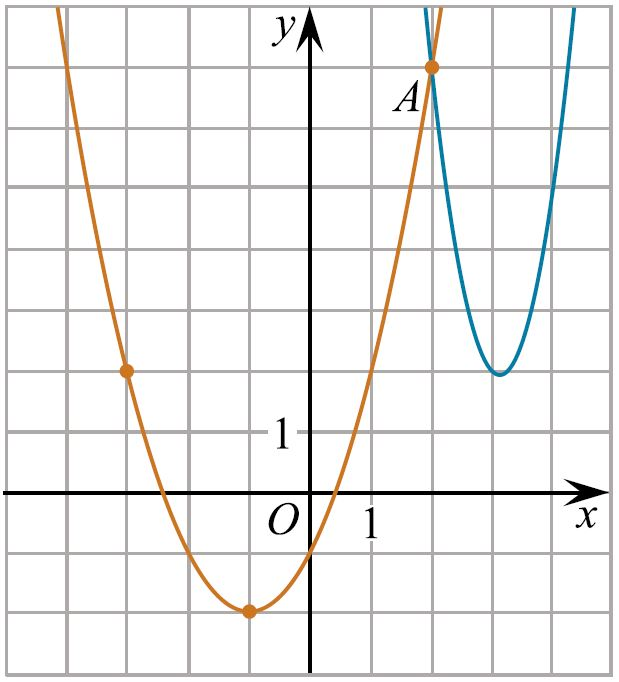
\includegraphics[align=t, width=\linewidth]{../pics/G112M3C1-10}
		\end{minipage}
		\item %1 LOGARIFM
		\begin{minipage}[t]{\bodywidth}
			На рисунке изображен график функции \(f(x) = b+\log_ax \). Найдите \(f(32)\).
		\end{minipage}
		\hspace{0.02\linewidth}
		\begin{minipage}[t]{\picwidth}
			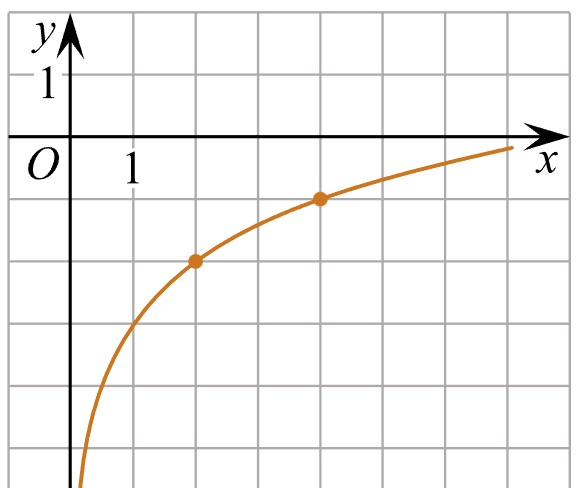
\includegraphics[align=t, width=\linewidth]{../pics/G111M8L1-1}
		\end{minipage}
		\item %1 s golovi
		\begin{minipage}[t]{\bodywidth}
			На рисунке изображен график функции \(f(x) = \dfrac{ x^2 }{ a }+bx+c \), где числа \(a, b, c\) --- целые. Найдите значение \(f(3,5)\).
		\end{minipage}
		\hspace{0.02\linewidth}
		\begin{minipage}[t]{\picwidth}
			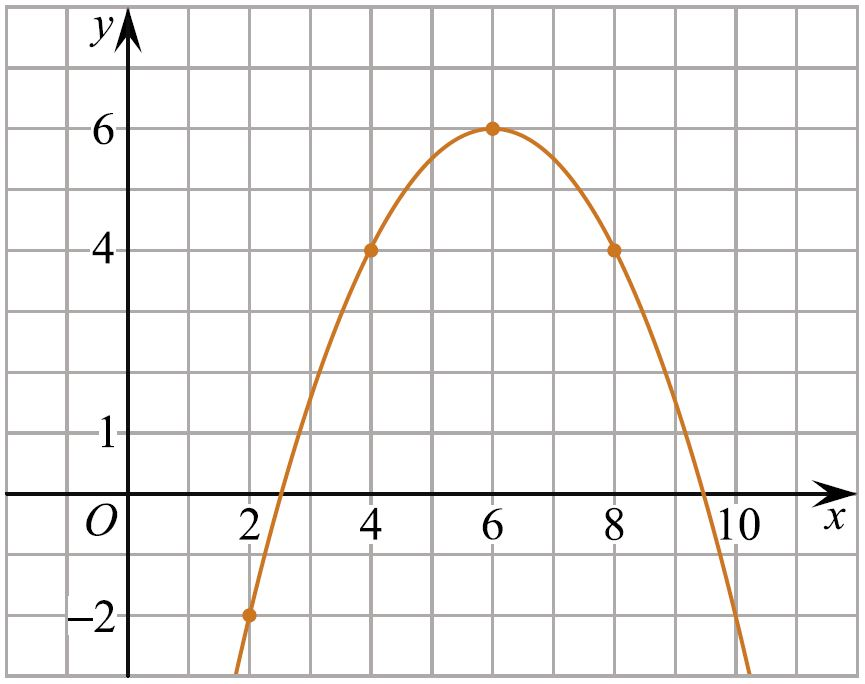
\includegraphics[align=t, width=\linewidth]{../pics/G112M3C1-6}
		\end{minipage}
	\end{listofex}
\end{class}
%END_FOLD

%BEGIN_FOLD % ====>>_____ Занятие 2 _____<<====
\begin{class}[number=2]
	\begin{listofex}
		\item Занятие 2
	\end{listofex}
\end{class}
%END_FOLD

%BEGIN_FOLD % ====>>_ Домашняя работа 1 _<<====
\begin{homework}[number=1]
	\begin{listofex}
		\item Домашняя работа 1
	\end{listofex}
\end{homework}
%END_FOLD

%BEGIN_FOLD % ====>>_____ Занятие 3 _____<<====
\begin{class}[number=3]
	\begin{listofex}
		\item Занятие 3 
	\end{listofex}
\end{class}
%END_FOLD

%BEGIN_FOLD % ====>>_____ Занятие 4 _____<<====
\begin{class}[number=4]
	\begin{listofex}
		\item Занятие 4
	\end{listofex}
\end{class}
%END_FOLD

%BEGIN_FOLD % ====>>_ Домашняя работа 2 _<<====
\begin{homework}[number=2]
	\begin{listofex}
		\item Домашняя работа 2
	\end{listofex}
\end{homework}
%END_FOLD

%BEGIN_FOLD % ====>>_____ Занятие 5 _____<<====
\begin{class}[number=5]
	\begin{listofex}
		\item Занятие 5
	\end{listofex}
\end{class}
%END_FOLD

%BEGIN_FOLD % ====>>_____ Занятие 6 _____<<====
\begin{class}[number=6]
	\begin{listofex}
		\item Занятие 6
	\end{listofex}
\end{class}
%END_FOLD

%BEGIN_FOLD % ====>>_ Домашняя работа 3 _<<====
\begin{homework}[number=3]
	\begin{listofex}
		\item Домашняя работа 3
	\end{listofex}
\end{homework}
%END_FOLD

%BEGIN_FOLD % ====>>_____ Занятие 7 _____<<====
\begin{class}[number=7]
	\title{Подготовка к проверочной}
	\begin{listofex}
		\item Занятие 7
	\end{listofex}
\end{class}
%END_FOLD

=%BEGIN_FOLD % ====>>_ Проверочная работа _<<====
\begin{exam}
	\begin{listofex}
		\item Проверочная
	\end{listofex}
\end{exam}
%END_FOLD